\subsection*{UI Design} \label{UI_Design}
A well-designed user interface is a critical component of any audio DSP project, particularly when utilizing a Nextion or similar screen. The user interface should be designed with simplicity in mind to ensure it is accessible to everyone who uses it. One of the primary goals of a good UI is to ensure that it is intuitive and easy to remember, so that users can begin using the product without feeling frustrated or overwhelmed.

\subsubsection*{Consistent}
The UI should maintain a consistent style throughout, so that each new menu or dial looks and feels the same as every other menu. This ensures that using the menus is easy and recognizable, even for new users.

\subsubsection*{Readability}
Text shown in menus should not be cut off, as this can be frustrating for users trying to read it. Short sentences are preferred to keep the menus clean and easy to read. When a sentence is cut off by the edge of the screen, users may struggle to figure out what it says, leading to confusion and frustration.

\subsubsection*{Feedback}
Finally, it is important to provide feedback to the user when the system needs time to load in certain elements or execute specific settings. Without feedback, users may become frustrated and begin clicking buttons multiple times, which can lead to software errors. By providing clear feedback during loading processes, users are more likely to remain patient and avoid potential issues.

\section{Nextion screen}

For this project a Nextion screen is used. This screen can easily be programmed. It comes with software which is image based instead of code based. Images can be inserted and "invisible" buttons can be used to make menus out of the inserted images.

This is a neat way to work because now it is possible to create images in Photoshop or a similar application to use for the whole menu design

\subsection{Designing the UI}
The design was started with a diagram with all the necessary screens and information so that is was clear what menus should be in the DSP. 

\begin{figure}[ht]
    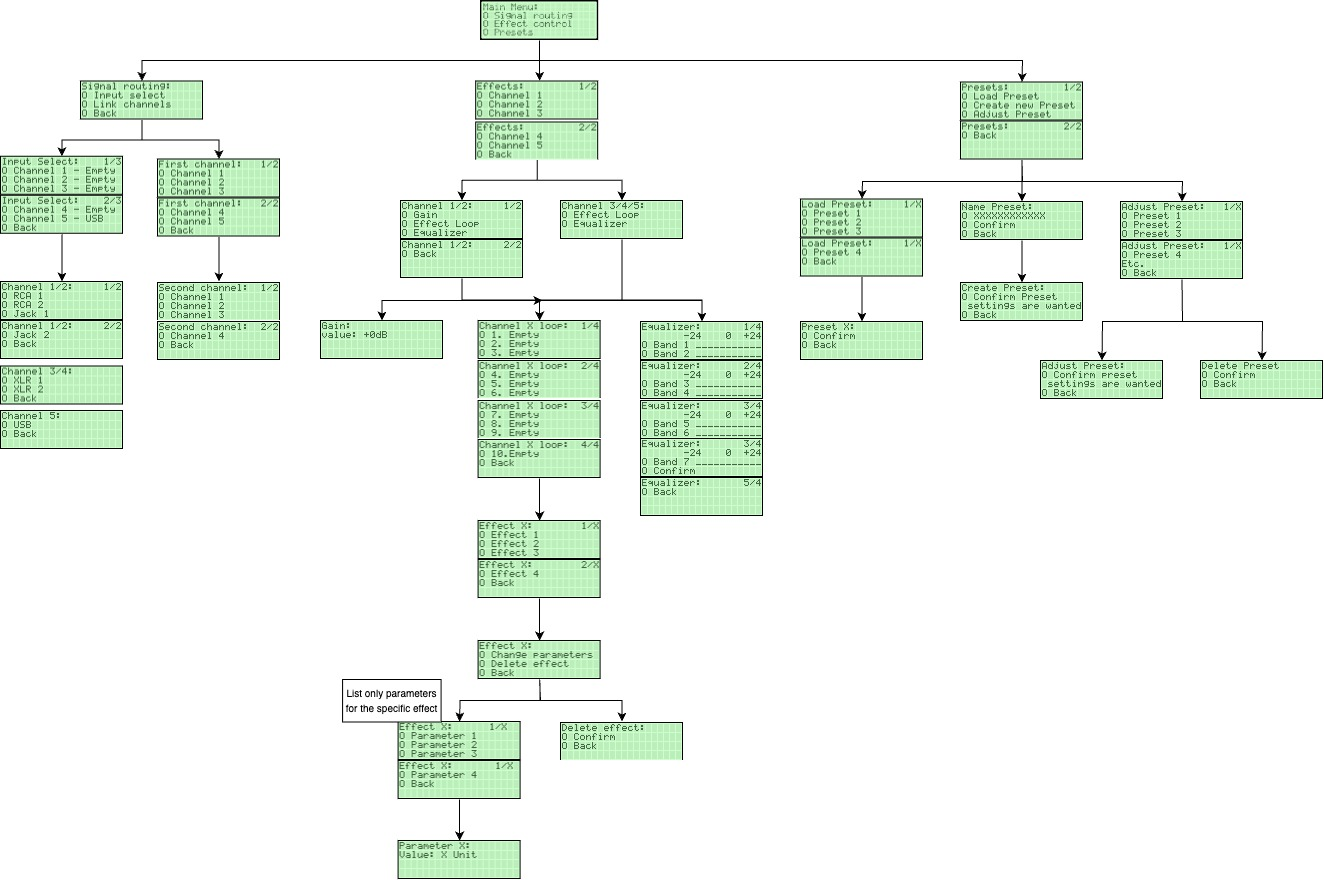
\includegraphics[width=\linewidth]{functionbasedUI}
    \caption{Function Based UI Design for a liquidCrystal screen}
    \label{fig:functionbasedUI}
\end{figure}

This UI is easy to understand when first using the DSP. Options and settings are easy to find from the first menu screen. While a channel based UI is unclear because every option is branched off from the channel select.
\par
\noindent The UI is designed using Adobe Photoshop. Bright but matching colors are used to indicate certain buttons. Using the Nextion screen software, invisible buttons are placed over the Photoshop pictures to make it a usable menu. The menu follows the liquidCrystal function based UI schematic. (see \ref{fig:functionbasedUI})

\begin{figure}[ht]
    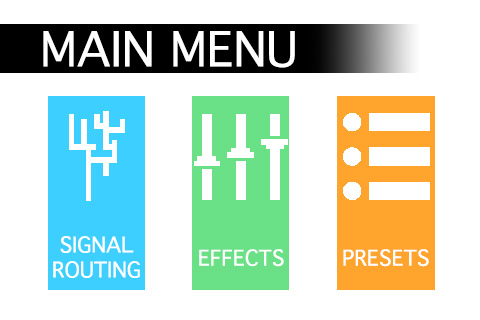
\includegraphics[width=0.8\textwidth]{MainMenu1}
    \caption{Main menu design}
    \label{fig:mainmenu}
\end{figure}

\begin{figure}[ht]
    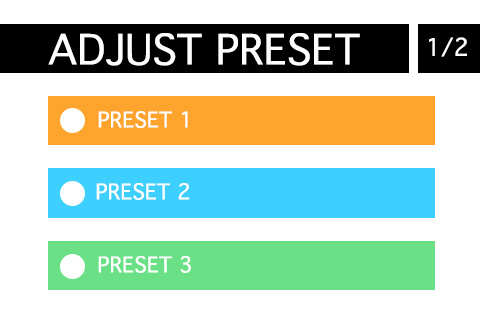
\includegraphics[width=0.8\textwidth]{adjustpreset1-2}
    \caption{Other menu screen, other ones are similar to this one}
    \label{fig:adjustpresetmenu}
\end{figure}


